\chapter{De los imanes de Ising a la--criticidad de los fluidos}

\lectureoverview{La transición líquido--gas puede abordarse por una vía inesperada. Primero completamos el tratamiento de campo medio del imán de Ising e identificamos su línea de coexistencia y su punto crítico; después reinterpretamos un espín hacia arriba como un sitio ocupado de la red. El gas reticular resultante tiene exclusión de núcleo duro, atracción de corto alcance y un potencial químico controlado por el campo magnético, y presenta exactamente el mismo diagrama de fases. El curso formal concluye con el comportamiento crítico y la universalidad. En una conversación aparte después de la clase se examina qué entienden los físicos por ajuste fino, cómo pueden intervenir los efectos de selección en una explicación y por qué ese razonamiento solo resulta útil si se combina con un mecanismo y con posibles pruebas.}

\section{Por qué el agua empieza a hervir con un imán}

El agua hirviendo es el fenómeno familiar que queremos entender: un líquido se transforma en gas y su densidad cambia bruscamente. La vía habitual pasa por la ecuación de van der Waals. Aquí seguiremos otra. Volveremos al imán de Ising, completaremos su descripción de campo medio y descubriremos que el mismo modelo puede interpretarse como un fluido.

Esto es más que una analogía sugerente. Una vez traducidas correctamente las variables, el imán de Ising y el gas reticular son el mismo sistema de mecánica estadística. La magnetización se convierte en densidad de partículas, el campo magnético externo en potencial químico y la línea de coexistencia magnética en la línea de coexistencia líquido--gas. Esta traducción explica por qué dos sistemas materiales aparentemente distintos pueden presentar el mismo comportamiento crítico.

El campo medio no proporciona respuestas numéricas exactas en dimensiones bajas. En una dimensión, incluso predice una transición que la solución exacta descarta. Aquí su valor es estructural. En dos y tres dimensiones revela el parámetro de orden correcto, las fases en competencia, el extremo crítico y cómo un sesgo infinitesimal selecciona una de las fases. En tres dimensiones, donde cada sitio tiene seis vecinos más próximos, sustituir esos vecinos por su valor medio ya proporciona una imagen cualitativa útil.

\section{El balance de energía de Ising}

Coloquemos un espín de dos estados en cada sitio de una red hipercúbica,
\begin{equation}
\sigma_i=\pm1.
\end{equation}
Usamos el hamiltoniano
\begin{equation}
\mathcal H
=-J\sum_{\langle ij\rangle}\sigma_i\sigma_j
+h\sum_i\sigma_i,
\qquad J>0.
\label{eq:ising-hamiltonian}
\end{equation}
La notación importa. La primera suma recorre los \emph{enlaces} entre vecinos más próximos; la segunda, los \emph{sitios}. Cada enlace se cuenta una sola vez, no una vez desde cada extremo.

Para un solo enlace,
\begin{equation}
E_{ij}=-J\sigma_i\sigma_j.
\end{equation}
Los espines paralelos tienen energía \(-J\), mientras que los antiparalelos tienen energía \(+J\). Por tanto, romper un enlace cuesta
\begin{equation}
\Delta E_{\rm bond}=+J-(-J)=2J.
\label{eq:broken-bond}
\end{equation}
El valor \(2J\), y no ninguna de las energías absolutas del enlace, es lo que determina los pesos de Boltzmann relativos. Podríamos sumar una constante a cada configuración sin cambiar ninguna probabilidad.

\begin{classroomqa}
\audiencequestion{¿Por qué hay dos sumas distintas en el hamiltoniano?}
\lecturerresponse{La energía de intercambio corresponde a un par de sitios vecinos, así que se suma sobre los enlaces \(\langle ij\rangle\). El campo actúa por separado sobre cada espín, así que se suma sobre los sitios \(i\). Confundir ambos recuentos introduce precisamente los factores de dos que serán importantes en el campo medio. \lecturetimestamp{00:08:04--00:08:45}}
\end{classroomqa}

\begin{classroomqa}
\audiencequestion{¿Aumentar \(J\) hace simplemente que todas las energías sean más negativas?}
\lecturerresponse{Aumenta la diferencia entre las configuraciones alineadas y las desalineadas. El cero de energía es arbitrario; la afirmación física es que romper un enlace cuesta \(2J\). Por tanto, un valor positivo mayor de \(J\) hace menos favorable el desorden térmico a temperatura fija. \lecturetimestamp{00:08:47--00:10:17}}
\end{classroomqa}

En una red hipercúbica infinita o periódica de \(d\) dimensiones, cada sitio tiene \(2d\) vecinos. Al contar desde los \(N\) sitios, cada enlace se cuenta dos veces, de modo que
\begin{equation}
N_{\rm links}=\frac{(2d)N}{2}=dN.
\label{eq:number-links}
\end{equation}
Por consiguiente, una configuración alineada tiene energía de intercambio \(-JdN\). Los sitios de frontera modifican este valor en un término superficial, despreciable frente a \(N\) en el límite termodinámico. Los dos estados completamente alineados son degenerados cuando \(h=0\).

El término de campo fija una convención de signo que mantendremos de manera coherente. En la ecuación~\eqref{eq:ising-hamiltonian}, un valor positivo de \(h\) asigna una energía menor por sitio a \(\sigma=-1\). Así, \(h>0\) favorece la magnetización negativa, mientras que \(h<0\) favorece la magnetización positiva. Se puede invertir esta convención escribiendo \(-h\sum_i\sigma_i\); nada físico cambia, pero entonces hay que invertir todos los signos posteriores.

\begin{classroomqa}
\audiencequestion{¿Dónde aparece la temperatura si el hamiltoniano solo contiene \(J\) y \(h\)?}
\lecturerresponse{La temperatura entra mediante el factor de Boltzmann \(e^{-\beta\mathcal H}\), con \(\beta=1/T\) en unidades \(k_{\rm B}=1\). Por tanto, las cantidades adimensionales son \(\beta J\) y \(\beta h\). \lecturetimestamp{00:13:07--00:13:43}}
\end{classroomqa}

\section{Un espín en el campo medio de sus vecinos}

Elijamos un espín lejos de la frontera. Tiene \(2d\) vecinos más próximos. En la aproximación de campo medio, cada vecino fluctuante se sustituye por el mismo valor medio,
\begin{equation}
m=\expect{\sigma}.
\end{equation}
La energía de intercambio que involucra al espín elegido \(\sigma\) queda entonces
\begin{equation}
-J\sigma\sum_{\text{\(2d\) neighbors}}\sigma_j
\;\longrightarrow\;-2dJm\,\sigma.
\end{equation}
Al añadir el campo externo se obtiene la energía efectiva de un espín,
\begin{equation}
\mathcal H_{\rm mf}(\sigma)=(-2dJm+h)\sigma.
\label{eq:mean-field-one-spin}
\end{equation}
El factor \(2d\) es esencial. Es fácil omitirlo al escribir el esquema del espín central, y se restituyó explícitamente durante la derivación en la pizarra.

\begin{figure}[ht]\centering
\includegraphics[width=0.84\textwidth]{lecture_10_figure_02.png}\caption{Un espín central rodeado por sus vecinos en la aproximación de campo medio, junto con la energía de un espín y la ecuación de autoconsistencia en desarrollo.}\lectureframe{00:17:57}\end{figure}

La función de partición de un espín es
\begin{align}
z_{\rm mf}
&=\sum_{\sigma=\pm1}
\exp\!\left[-\beta(-2dJm+h)\sigma\right] \\
&=2\cosh\!\left[\beta(2dJm-h)\right].
\end{align}
Su espín medio es
\begin{align}
\expect{\sigma}
&=\frac{\sum_{\sigma=\pm1}\sigma
 e^{\beta(2dJm-h)\sigma}}
{\sum_{\sigma=\pm1}e^{\beta(2dJm-h)\sigma}} \\
&=\tanh\!\left[\beta(2dJm-h)\right].
\end{align}
Pero se supone que el espín elegido es representativo de los vecinos cuyo valor medio hemos llamado \(m\). Por tanto, la autoconsistencia exige que
\begin{equation}
\boxed{m=\tanh\!\left[\beta(2dJm-h)\right].}
\label{eq:mean-field-self-consistency}
\end{equation}
Esta única ecuación no lineal es la reducción de campo medio del problema de muchos espines.

\begin{classroomqa}
\audiencequestion{¿Por qué el promedio de la izquierda es el mismo \(m\) que se asignó a cada vecino?}
\lecturerresponse{Esa igualdad es la aproximación. Suponemos un estado homogéneo en el volumen, sustituimos el entorno real por su promedio, calculamos el espín central en ese entorno y exigimos que el promedio calculado reproduzca el entorno supuesto. Una solución es un estado homogéneo autoconsistente. \lecturetimestamp{00:16:28--00:18:00}}
\end{classroomqa}

Introduzcamos
\begin{equation}
y=2\beta dJm.
\label{eq:y-definition}
\end{equation}
Como \(\beta=1/T\),
\begin{equation}
m=\frac{yT}{2dJ},
\end{equation}
y la ecuación~\eqref{eq:mean-field-self-consistency} se convierte en
\begin{equation}
\boxed{\frac{yT}{2dJ}=\tanh(y-\beta h).}
\label{eq:reduced-mean-field}
\end{equation}

\begin{figure}[ht]\centering
\includegraphics[width=0.82\textwidth]{lecture_10_figure_03.png}\caption{La ecuación de autoconsistencia reducida tras introducir \(y=2\beta dJm\), lista para resolverse gráficamente.}\lectureframe{00:24:42}\end{figure}

\begin{classroomqa}
\audiencequestion{¿Por qué aparece el campo como \(y-\beta h\) y qué espín favorece un campo positivo?}
\lecturerresponse{Nuestro hamiltoniano contiene \(+h\sigma\). Por tanto, su exponente de Boltzmann es \(\beta(2dJm-h)\sigma\), de modo que la tangente hiperbólica contiene \(y-\beta h\). Un valor positivo de \(h\) favorece \(\sigma=-1\). Si, en cambio, se define el hamiltoniano con \(-h\sigma\), cambia el signo de cada aparición de \(h\) y el diagrama de fases se refleja horizontalmente. \lecturetimestamp{00:18:17--00:20:00}}
\end{classroomqa}

\section{Soluciones gráficas y punto de Curie}

Fijemos \(h=0\). Hay que encontrar las intersecciones de
\begin{equation}
\frac{T}{2dJ}y
\qquad\text{and}\qquad
\tanh y.
\end{equation}
La primera es una recta que pasa por el origen; la segunda, una curva impar que se satura. A temperaturas altas, la recta es pronunciada y la única intersección es \(y=0\), por lo que \(m=0\). Al bajar la temperatura, la recta se hace menos pronunciada. Se alcanza la temperatura crítica cuando la recta y la tangente hiperbólica son tangentes en el origen.

\begin{figure}[ht]\centering
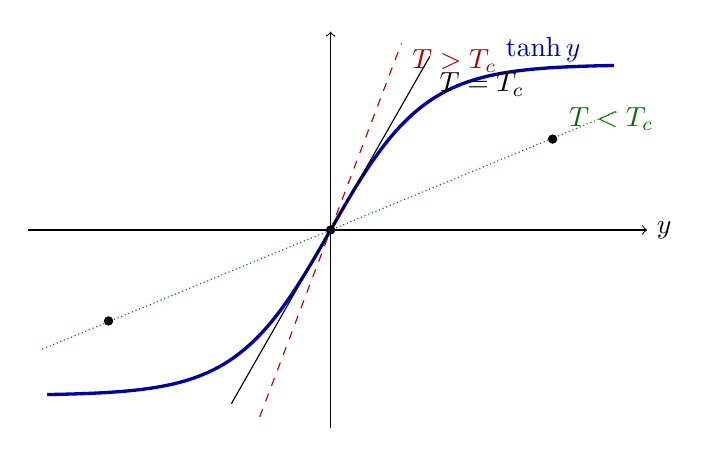
\begin{tikzpicture}[x=1.2cm,y=2.1cm]
\draw[->] (-3.2,0) -- (3.35,0) node[right] {$y$};
\draw[->] (0,-1.2) -- (0,1.2);
\draw[very thick,blue!65!black,domain=-3:3,samples=120]
  plot (\x,{tanh(\x)});
\node[blue!65!black,above] at (2.25,0.96) {$\tanh y$};
\draw[dashed,red!70!black] (-0.75,-1.13) -- (0.75,1.13);
\node[red!70!black,right] at (0.76,1.02) {$T>T_c$};
\draw[black] (-1.05,-1.05) -- (1.05,1.05);
\node[right] at (1.05,0.88) {$T=T_c$};
\draw[densely dotted,green!45!black] (-3.05,-0.72) -- (3.05,0.72);
\node[green!45!black,right] at (2.42,0.67) {$T<T_c$};
\fill (-2.35,-0.55) circle (1.7pt);
\fill (0,0) circle (1.7pt);
\fill (2.35,0.55) circle (1.7pt);
\end{tikzpicture}\caption{La ecuación de campo medio con campo nulo. Por debajo de \(T_c\), las dos intersecciones no nulas representan las fases magnetizadas estables; la solución nula sigue estando presente algebraicamente, pero es inestable.}\label{fig:mean-field-intersections}\end{figure}

Como
\begin{equation}
\left.\frac{d}{dy}\tanh y\right|_{y=0}=1,
\end{equation}
la condición de tangencia es
\begin{equation}
\frac{T_c}{2dJ}=1.
\end{equation}
Por tanto, el campo medio predice
\begin{equation}
\boxed{T_c^{\rm MF}=2dJ.}
\label{eq:sm10-mean-field-tc}
\end{equation}
Por debajo de esta temperatura hay dos soluciones estables no nulas \(\pm m_0(T)\). La solución \(m=0\) todavía satisface la ecuación, pero ya no es un equilibrio estable. El sistema elige una de las dos fases magnetizadas relacionadas por simetría.

\begin{classroomqa}
\audiencequestion{¿Es esta la temperatura de Curie?}
\lecturerresponse{Sí. En un ferromagneto, la temperatura a la que desaparece la magnetización espontánea se denomina convencionalmente temperatura de Curie. Aquí \(2dJ\) es su valor en la aproximación de campo medio, no un resultado exacto en dimensiones bajas. \lecturetimestamp{00:28:19--00:28:57}}
\end{classroomqa}

Cerca de la transición, desarrollamos la tangente hiperbólica:
\begin{equation}
\tanh y=y-\frac{y^3}{3}+O(y^5).
\end{equation}
Para \(h=0\), la ecuación~\eqref{eq:reduced-mean-field} da
\begin{equation}
\left(1-\frac{T}{T_c}\right)y-\frac{y^3}{3}+O(y^5)=0.
\end{equation}
Por tanto, las ramas no nulas se comportan como
\begin{equation}
y^2\simeq3\left(1-\frac{T}{T_c}\right),
\qquad
m\propto(T_c-T)^{1/2}.
\label{eq:mf-beta-exponent}
\end{equation}
La raíz cuadrada es un exponente crítico de campo medio. Su valor preciso no se conservará en dimensiones bajas, pero sí lo hará la anulación continua del parámetro de orden en el extremo.

\section{El plano de temperatura--campo y la selección de rama}

El material fija \(J\); el experimentador puede variar \(T\) y \(h\). Por eso es natural dibujar un diagrama de fases en el plano \(T\)--\(h\). Por debajo de \(T_c\), un campo arbitrariamente pequeño selecciona una de las dos ramas magnetizadas. Con nuestra convención, \(h<0\) selecciona \(m>0\), mientras que \(h>0\) selecciona \(m<0\).

A temperatura cero, los espines están completamente alineados, así que \(m=\pm1\). A temperatura alta, el promedio con campo nulo es \(m=0\). Al aproximarse al punto crítico a lo largo de \(h=0\), la magnitud \(m_0(T)\) disminuye continuamente hasta cero. Sin embargo, a cualquier \(T<T_c\) fija, cruzar \(h=0\) provoca un cambio discontinuo de \(+m_0(T)\) a \(-m_0(T)\).

\begin{figure}[ht]\centering
\includegraphics[width=0.90\textwidth]{lecture_10_figure_06.png}\caption{La línea de coexistencia en el plano \(T\)--\(h\) y las ramas de magnetización a temperatura fija por debajo de \(T_c\).}\lectureframe{00:39:30}\end{figure}

\begin{figure}[ht]\centering
\resizebox{\linewidth}{!}{%
\begin{tikzpicture}[x=1.25cm,y=1.15cm]
\begin{scope}
\draw[->] (-2.45,0) -- (2.55,0) node[right] {$h$};
\draw[->] (0,0) -- (0,3.7) node[above] {$T$};
\draw[very thick,red!70!black] (0,0) -- (0,2.35);
\fill[red!70!black] (0,2.35) circle (2.3pt);
\node[right] at (0.08,2.35) {$T_c$};
\node at (-1.25,1.05) {$m>0$};
\node at (1.25,1.05) {$m<0$};
\draw[->,rounded corners,blue!65!black] (-1.65,0.85) -- (-1.65,3.02)
 -- (1.65,3.02) -- (1.65,0.85);
\node[blue!65!black] at (0,3.35) {continuous path};
\end{scope}
\begin{scope}[xshift=7.0cm,yshift=1.55cm]
\draw[->] (-2.5,0) -- (2.5,0) node[right] {$h$};
\draw[->] (0,-1.35) -- (0,1.4) node[above] {$m$};
\draw[very thick,blue!65!black]
  (-2.2,1.05) .. controls (-0.75,1.03) and (-0.2,0.75) .. (-0.08,0.62);
\draw[very thick,blue!65!black]
  (0.08,-0.62) .. controls (0.2,-0.75) and (0.75,-1.03) .. (2.2,-1.05);
\draw[dashed] (0,0.62) -- (0,-0.62);
\fill (0,0.62) circle (1.8pt);
\fill (0,-0.62) circle (1.8pt);
\node at (0,-1.75) {\(T<T_c\)};
\end{scope}
\end{tikzpicture}}\caption{A \(T<T_c\) fija, la magnetización salta al cruzar la línea de coexistencia. En el plano completo de dos parámetros, en cambio, se pueden conectar las dos fases continuamente rodeando el punto crítico.}\label{fig:ising-phase-plane}\end{figure}

\begin{classroomqa}
\audiencequestion{¿Qué ocurre si el campo es exactamente cero por debajo de \(T_c\)?}
\lecturerresponse{El sistema infinito ideal tiene dos fases puras igualmente favorables. Cualquier sesgo residual infinitesimal, condición de frontera o fluctuación asociada a la preparación selecciona una de ellas. En nuestra convención de signos, la discontinuidad termodinámica se expresa mediante los dos límites laterales \(m(T,0^-)=+m_0(T)\) y \(m(T,0^+)=-m_0(T)\). \lecturetimestamp{00:35:04--00:37:10}}
\end{classroomqa}

\begin{classroomqa}
\audiencequestion{¿Es esto lo mismo que la histéresis?}
\lecturerresponse{La histéresis se refiere a la metaestabilidad y al retraso, dependiente de la historia, con que un sistema real cambia de rama. Está relacionada, pero requiere una dinámica que va más allá del diagrama de fases de equilibrio y que aquí no desarrollamos. \lecturetimestamp{00:37:11--00:37:20}}
\end{classroomqa}

\begin{classroomqa}
\audiencequestion{¿Se pueden conectar las fases positiva y negativa sin cruzar una discontinuidad?}
\lecturerresponse{Sí. Aumentemos la temperatura por encima de \(T_c\), cambiemos allí el signo del campo y volvamos a bajar la temperatura. Esa trayectoria rodea el extremo y la magnetización cambia continuamente. El salto es inevitable únicamente al cruzar \(h=0\) a \(T<T_c\) fija. \lecturetimestamp{00:37:20--00:38:15}}
\end{classroomqa}

\begin{classroomqa}
\audiencequestion{¿La magnetización se aproxima a cero siempre que \(h\) se aproxime a cero?}
\lecturerresponse{No a una temperatura genérica por debajo de \(T_c\). Allí, los límites laterales son distintos de cero. La magnetización espontánea se aproxima a cero solo cuando la temperatura misma se aproxima a la temperatura crítica. \lecturetimestamp{00:38:29--00:39:45}}
\end{classroomqa}

\section{Una caja permeable y el potencial químico}

Ahora dejamos los imanes y empezamos de nuevo con partículas. Imaginemos una región cuya energía potencial es menor que la del espacio circundante. Las paredes son permeables: las partículas pueden entrar y salir. Si la energía en el interior es menor en una cantidad \(\mu\), la ocupación interior recibe un factor de Boltzmann relativo \(e^{\beta\mu}\). Al profundizar o elevar el pozo cambia el número medio de partículas en la caja.

\begin{figure}[ht]\centering
\includegraphics[width=0.84\textwidth]{lecture_10_figure_07.png}\caption{La representación de una caja permeable mediante un pozo de potencial. La diferencia de energía entre el interior y el exterior determina la preferencia de las partículas por ocupar la caja.}\lectureframe{00:41:30}\end{figure}

\begin{figure}[ht]\centering
\resizebox{\linewidth}{!}{%
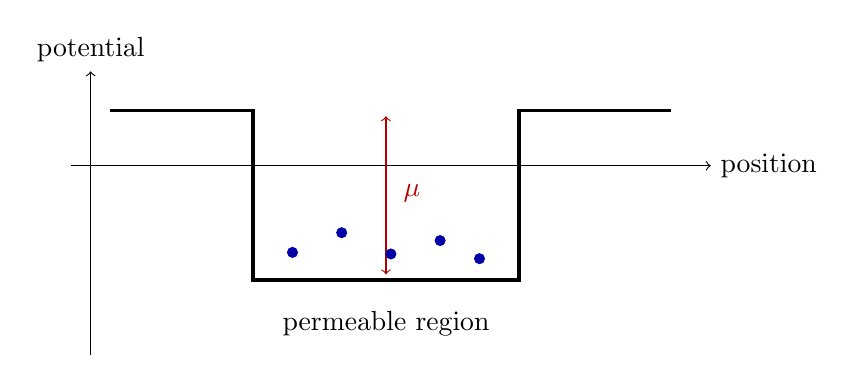
\begin{tikzpicture}[x=1.25cm,y=1.0cm]
\draw[->] (-3.2,0) -- (3.3,0) node[right] {position};
\draw[->] (-3.0,-2.4) -- (-3.0,1.2) node[above] {potential};
\draw[very thick] (-2.8,0.7) -- (-1.35,0.7)
 -- (-1.35,-1.45) -- (1.35,-1.45) -- (1.35,0.7) -- (2.9,0.7);
\draw[<->,red!70!black] (0,0.63) -- (0,-1.38);
\node[right,red!70!black] at (0.08,-0.35) {$\mu$};
\foreach \x/\y in {-0.95/-1.1,-0.45/-0.85,0.05/-1.12,0.55/-0.95,0.95/-1.18}
  \fill[blue!65!black] (\x,\y) circle (2pt);
\node at (0,-2.0) {permeable region};
\end{tikzpicture}}\caption{Al cambiar el desplazamiento del potencial cambia la preferencia por el número de partículas. En la descripción gran canónica, ese desplazamiento se representa mediante el potencial químico.}\end{figure}

Este experimento mental concreta el concepto de potencial químico. Es una ventaja energética por cada partícula añadida, con respecto a un reservorio. Si varias especies pueden atravesar la pared, cada una tiene su propio potencial químico. Una caja sellada es distinta: en ese caso \(N\) se mantiene fijo y el potencial químico se infiere termodinámicamente, en vez de imponerse mediante el intercambio con un reservorio.

\begin{classroomqa}
\audiencequestion{¿La profundidad del pozo es literalmente el potencial químico?}
\lecturerresponse{Es una realización mecánica directa de una diferencia de potencial químico. Bajar en \(\mu\) todos los niveles de una partícula en el interior aporta \(-\mu N\) a la energía y, por tanto, \(+\beta\mu N\) al exponente de Boltzmann. Solo importan las diferencias de potencial químico. \lecturetimestamp{00:44:49--00:45:40}}
\end{classroomqa}

Como las partículas pueden entrar y salir, la suma de partición debe incluir todos los números de partículas:
\begin{equation}
\Xi(T,\mu)
=\sum_{N=0}^{\infty}\;\sum_{\mathcal C_N}
\exp\!\left[-\beta E(\mathcal C_N)+\beta\mu N\right].
\label{eq:grand-partition}
\end{equation}
La suma interior recorre las configuraciones con un valor especificado de \(N\); la suma exterior recorre el propio \(N\). El peso gran canónico también puede escribirse como \(e^{-\beta(E-\mu N)}\).

\begin{figure}[ht]\centering
\includegraphics[width=0.88\textwidth]{lecture_10_figure_08.png}\caption{La caja permeable y la suma gran canónica sobre el número de partículas y las configuraciones.}\lectureframe{00:47:15}\end{figure}

\begin{classroomqa}
\audiencequestion{¿Qué cambia cuando se sella la caja?}
\lecturerresponse{El número de partículas deja de fluctuar. Entonces se usa la función de partición canónica a \(N\) fijo. En la caja permeable, \(N\) es una variable termodinámica cuyo valor medio controla \(\mu\). \lecturetimestamp{00:45:42--00:47:50}}
\end{classroomqa}

A temperatura fija, variar \(\mu\) normalmente cambia la densidad de forma continua. Por debajo de una temperatura crítica, en cambio, puede provocar un salto abrupto. Ese es el fenómeno de los fluidos que queremos estudiar. Para obtenerlo a nivel microscópico, las partículas necesitan dos propiedades: no deben poder ocupar el mismo lugar y deben atraerse a corto alcance.

\section{De los espines a un gas reticular}

Conservemos la red, pero reinterpretemos sus dos estados. Definamos un número de ocupación
\begin{equation}
n_i=\frac{1+\sigma_i}{2}
=
\begin{cases}
0,&\sigma_i=-1,\\
1,&\sigma_i=+1.
\end{cases}
\label{eq:occupation-map}
\end{equation}
Un sitio vacío tiene espín hacia abajo; uno ocupado, espín hacia arriba. Como \(n_i\) solo puede valer cero o uno, se prohíbe la doble ocupación. Por tanto, la propia red proporciona el núcleo duro.

\begin{figure}[ht]\centering
\includegraphics[width=0.84\textwidth]{lecture_10_figure_04.png}\caption{La identificación con el gas reticular empieza con \(\sigma=-1\) como sitio vacío; \(\sigma=+1\) corresponde entonces a un sitio ocupado.}\lectureframe{00:53:45}\end{figure}

Empecemos con la red vacía, toda ella en el estado \(\sigma=-1\). Todos los enlaces están alineados y tienen energía \(-J\). Podemos restar esa energía constante del vacío. Coloquemos ahora una partícula en un sitio de una red bidimensional. El espín correspondiente cambia a \(+1\) y rompe cuatro enlaces. Cada enlace roto cuesta \(2J\), así que
\begin{equation}
\Delta E_1=4(2J)=8J.
\label{eq:one-particle-cost}
\end{equation}
Dos partículas muy separadas rompen ocho enlaces y cuestan \(16J\). Si ocupan sitios vecinos, el enlace entre ellas vuelve a estar alineado. Solo se rompen seis enlaces del contorno, y el coste es
\begin{equation}
\Delta E_{2,\rm adjacent}=6(2J)=12J.
\end{equation}
Por tanto, al acercar las partículas la energía disminuye en
\begin{equation}
16J-12J=4J.
\label{eq:lattice-attraction}
\end{equation}
En la explicación oral, primero se describió el recuento como un ahorro de \(2J\) y luego se corrigió: un enlace compartido elimina dos contribuciones de enlaces rotos en el contorno, así que la atracción es de \(4J\).

\begin{figure}[ht]\centering
\includegraphics[width=0.84\textwidth]{lecture_10_figure_05.png}\caption{Recuento de enlaces en dos dimensiones: una partícula aislada cuesta \(8J\), dos partículas distantes cuestan \(16J\) y dos partículas adyacentes cuestan \(12J\).}\lectureframe{01:00:25}\end{figure}

El gas reticular ya tiene las dos propiedades moleculares necesarias. La ocupación binaria aporta exclusión de núcleo duro, y la interacción de intercambio aporta una atracción entre vecinos más próximos de intensidad \(4J\). El número de partículas puede fluctuar porque los cambios de espín modifican el número de sitios ocupados.

\subsection{El diccionario algebraico exacto}

El recuento de enlaces basta para ver la física, pero el cambio exacto de variables hace innegable la equivalencia. Sustituyamos
\begin{equation}
\sigma_i=2n_i-1
\end{equation}
en la ecuación~\eqref{eq:ising-hamiltonian}. Para un enlace,
\begin{equation}
\sigma_i\sigma_j
=4n_in_j-2n_i-2n_j+1.
\end{equation}
En una red regular de dimensión \(d\),
\begin{equation}
\sum_{\langle ij\rangle}(n_i+n_j)=2d\sum_i n_i.
\end{equation}
Por tanto,
\begin{align}
\mathcal H
&=-4J\sum_{\langle ij\rangle}n_in_j
+(4dJ+2h)\sum_i n_i+\text{constant}.
\label{eq:ising-as-lattice-gas}
\end{align}
Comparemos esto con el hamiltoniano convencional del gas reticular,
\begin{equation}
\mathcal H_{\rm lg}
=-\epsilon\sum_{\langle ij\rangle}n_in_j
-\mu\sum_i n_i+\text{constant}.
\label{eq:lattice-gas-hamiltonian}
\end{equation}
El diccionario es
\begin{equation}
\boxed{\epsilon=4J,\qquad
\mu=-(4dJ+2h).}
\label{eq:chemical-potential-map}
\end{equation}

\begin{figure}[ht]\centering
\includegraphics[width=0.88\textwidth]{lecture_10_figure_09.png}\caption{Los términos de intercambio y de campo junto al recuento de la energía de las partículas. El campo modifica la energía de inserción sin cambiar la atracción entre vecinos más próximos.}\lectureframe{01:04:30}\end{figure}

En dos dimensiones, una inserción aislada modifica la energía en
\begin{equation}
8J+2h=-\mu.
\end{equation}
El término \(8J\) proviene de los enlaces rotos; \(2h\), del cambio de un espín de \(-1\) a \(+1\). Por tanto, ajustar \(h\) permite ajustar el potencial químico y mantener fija la atracción \(4J\). El campo no es literalmente igual a \(\mu\), porque la energía de referencia de intercambio aporta el desplazamiento \(4dJ\).

\begin{classroomqa}
\audiencequestion{Si el campo controla el número de partículas, ¿por qué \(h\) no es simplemente el potencial químico?}
\lecturerresponse{Crear una partícula también rompe enlaces de intercambio con respecto al estado de referencia vacío. Por eso, el coeficiente convencional de \(-N\) es \(\mu=-(4dJ+2h)\), no solo \(-2h\). El desplazamiento depende de \(J\) y del número de coordinación. \lecturetimestamp{01:06:28--01:06:41}}
\end{classroomqa}

La densidad es igual de sencilla:
\begin{equation}
\rho=\expect{n_i}
=\frac{1+\expect{\sigma_i}}{2}
=\frac{1+m}{2}.
\label{eq:density-map}
\end{equation}
Así, \(m=-1\) corresponde a la red vacía, \(m=+1\) a la red completamente llena y \(m=0\) a la mitad de ocupación. El número total de partículas es \(N_{\rm p}=\sum_i n_i\); la densidad es \(N_{\rm p}/N\).

\begin{figure}[ht]\centering
\includegraphics[width=0.90\textwidth]{lecture_10_figure_10.png}\caption{La relación entre densidad \(\rho=(1+m)/2\) y la línea de coexistencia magnética.}\lectureframe{01:08:25}\end{figure}

\begin{classroomqa}
\audiencequestion{¿\((1+m)/2\) es el número de partículas o la densidad?}
\lecturerresponse{Es la ocupación media por sitio y, por tanto, la densidad reticular adimensional. Al multiplicarla por el número total de sitios se obtiene el número esperado de partículas. Es importante distinguir una densidad intensiva de un recuento extensivo. \lecturetimestamp{01:06:43--01:09:31}}
\end{classroomqa}

\section{El diagrama de fases magnético se convierte en el diagrama de fases del fluido}

Traduzcamos la figura~\ref{fig:ising-phase-plane} mediante las ecuaciones~\eqref{eq:chemical-potential-map} y \eqref{eq:density-map}. Por encima de \(T_c\), variar \(\mu\) cambia la densidad de manera continua. Por debajo de \(T_c\), cruzar el valor de coexistencia
\begin{equation}
\mu_{\rm coex}=-4dJ
\qquad(h=0)
\label{eq:coexistence-mu}
\end{equation}
provoca un salto de densidad entre un gas diluido y un líquido denso. En \(T_c\), las dos densidades coinciden y desaparece la discontinuidad.

\begin{figure}[ht]\centering
\includegraphics[width=0.92\textwidth]{lecture_10_figure_11.png}\caption{La línea de coexistencia de Ising interpretada como un diagrama de fases líquido--gas. El gas se encuentra del lado de baja densidad y el líquido, del lado de alta densidad; ambos pueden conectarse continuamente rodeando el extremo crítico.}\lectureframe{01:14:30}\end{figure}

\begin{figure}[ht]\centering
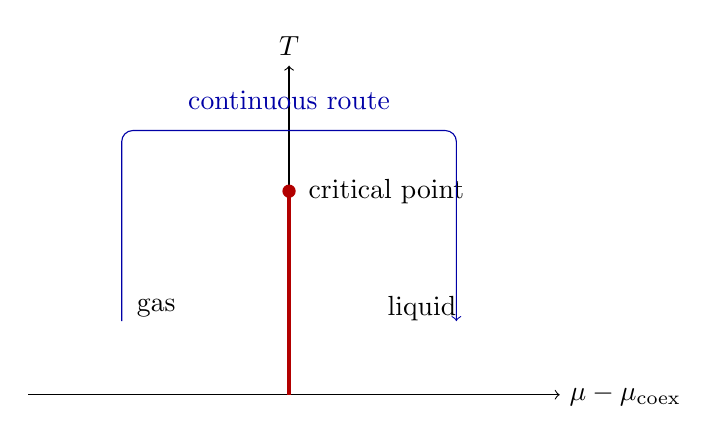
\begin{tikzpicture}[x=1.25cm,y=1.1cm]
\draw[->] (-2.65,0) -- (2.75,0) node[right] {$\mu-\mu_{\rm coex}$};
\draw[->] (0,0) -- (0,3.8) node[above] {$T$};
\draw[very thick,red!70!black] (0,0) -- (0,2.35);
\fill[red!70!black] (0,2.35) circle (2.4pt);
\node[right] at (0.1,2.35) {critical point};
\node at (-1.35,1.0) {gas};
\node at (1.35,1.0) {liquid};
\draw[->,blue!65!black,rounded corners]
 (-1.7,0.85) -- (-1.7,3.05) -- (1.7,3.05) -- (1.7,0.85);
\node[blue!65!black] at (0,3.4) {continuous route};
\end{tikzpicture}\caption{El líquido y el gas son fases distintas por debajo del extremo, pero en la región supercrítica no hay ninguna frontera singular que los separe.}\label{fig:liquid-gas-plane}\end{figure}

Esto identifica la conocida curva de ebullición. A presión fija, calentar un líquido hasta que cruce la coexistencia produce la ebullición. A temperatura fija, cambiar la presión o el potencial químico puede cruzar la misma frontera. Un vapor sobrecalentado o un líquido sobreenfriado son continuaciones metaestables más allá de la coexistencia de equilibrio; describir su duración exige estudiar la dinámica de nucleación, que queda fuera de esta construcción de equilibrio.

\begin{classroomqa}
\audiencequestion{¿Está representado el vapor de agua sobrecalentado en este diagrama de fases?}
\lecturerresponse{El diagrama de equilibrio identifica la frontera de coexistencia. Un estado sobrecalentado o sobresaturado es metaestable: persiste temporalmente en el lado desfavorable porque formar una gota crítica tiene un coste de energía libre interfacial. Aquí no calculamos este refinamiento cinético. \lecturetimestamp{01:12:19--01:12:29}}
\end{classroomqa}

\begin{classroomqa}
\audiencequestion{¿Cómo se varía el potencial químico en un fluido ordinario?}
\lecturerresponse{La caja con un pozo de potencial es el mecanismo de control teórico más claro. En el laboratorio es más habitual cambiar la presión, el volumen o el contacto con un reservorio; la termodinámica traduce entonces esos controles en un cambio del potencial químico. \lecturetimestamp{01:12:30--01:13:59}}
\end{classroomqa}

\begin{classroomqa}
\audiencequestion{Cuando cambia la densidad, ¿estamos cambiando el potencial molecular \(J\)?}
\lecturerresponse{No. Para una sustancia fija, \(J\) representa la atracción de corto alcance y permanece fijo en este modelo. Cambiar \(\mu\) modifica cuántos sitios están ocupados y, por tanto, la distribución de las separaciones intermoleculares. Cambiar \(J\) equivaldría a cambiar la sustancia microscópica o la interacción. \lecturetimestamp{01:14:50--01:15:41}}
\end{classroomqa}

\begin{classroomqa}
\audiencequestion{¿Es la temperatura crítica lo mismo que el punto de ebullición ordinario?}
\lecturerresponse{No. Un punto de ebullición se especifica a una presión elegida, así que se desplaza a lo largo de la curva de coexistencia cuando cambia la presión. La temperatura crítica es el único extremo por encima del cual el líquido y el gas dejan de estar separados por una frontera de fase. En este tratamiento del gas reticular no hemos derivado explícitamente la presión. \lecturetimestamp{01:15:42--01:17:02}}
\end{classroomqa}

Ya podemos enunciar el resultado central. El imán de Ising y el gas reticular no se limitan a tener diagramas parecidos: comparten una función de partición tras un cambio de variables y parámetros. A cada propiedad termodinámica singular de uno le corresponde una propiedad del otro:
\begin{equation}
\begin{array}{c|c}
\text{Ising magnet} & \text{lattice gas}\\ \hline
\sigma_i=\pm1 & n_i=0,1\\
m=\expect{\sigma} & \rho=(1+m)/2\\
h & \mu=-(4dJ+2h)\\
\text{aligned exchange} & \text{nearest-neighbor attraction}\\
h=0,\ T<T_c & \text{liquid--gas coexistence}\\
(T_c,0) & \text{critical endpoint}
\end{array}
\label{eq:ising-fluid-dictionary}
\end{equation}

\section{Exponentes críticos y universalidad}

Cerca de un punto crítico, las magnitudes termodinámicas suelen presentar singularidades de tipo ley de potencias. Con la temperatura reducida
\begin{equation}
t=\frac{T-T_c}{T_c},
\end{equation}
se escribe, esquemáticamente,
\begin{equation}
m\sim(-t)^{\beta_{\rm crit}},
\qquad
\chi\sim |t|^{-\gamma},
\qquad
\xi\sim |t|^{-\nu}.
\label{eq:critical-exponents}
\end{equation}
Aquí \(\beta_{\rm crit}\) es un exponente crítico, no la inversa de la temperatura. El campo medio da \(\beta_{\rm crit}=1/2\), pero las fluctuaciones modifican los exponentes por debajo de la dimensión crítica superior.

Los exponentes no tienen por qué ser enteros, ni tampoco tienen por qué ser todos irracionales: el modelo de Ising bidimensional tiene, como es bien sabido, varios exponentes racionales exactos, mientras que los valores del modelo tridimensional son números no triviales determinados con gran precisión mediante teoría y cálculo. La lección general es que los exponentes no vienen determinados, por lo común, por un análisis dimensional elemental.

Más sorprendente aún: a menudo los detalles microscópicos no los determinan. Los sistemas con la misma dimensión espacial, la misma simetría del parámetro de orden e interacciones suficientemente cortas pueden converger a la misma teoría crítica de largo alcance. Pertenecen a una \emph{clase de universalidad}. Tanto un ferromagneto uniaxial como el extremo líquido--gas de un fluido ordinario tienen un único parámetro de orden escalar y comparten la clase de universalidad de Ising en la misma dimensión.

\begin{classroomqa}
\audiencequestion{¿Las clases de universalidad forman una lista finita o discreta?}
\lecturerresponse{Hay muchas clases, organizadas según la dimensión, las simetrías, las leyes de conservación, el alcance de las interacciones y otros datos de largo alcance. En muchos casos conocidos, los puntos fijos y los conjuntos de exponentes son discretos, pero también hay sistemas con exponentes que varían continuamente. La afirmación prudente no es que el catálogo sea finito, sino que muchos sistemas microscópicamente distintos comparten los mismos datos de largo alcance. \lecturetimestamp{01:18:50--01:19:38}}
\end{classroomqa}

\begin{classroomqa}
\audiencequestion{Si el líquido y el gas coexisten, ¿qué los separa en un recipiente real?}
\lecturerresponse{Los separa una interfaz. La tensión superficial penaliza el área interfacial, mientras que la gravedad crea un gradiente vertical de potencial químico y suele situar el líquido, más denso, debajo del gas. Cuando la gravedad es despreciable, la geometría depende más directamente de la tensión superficial y de las condiciones de frontera. \lecturetimestamp{01:19:40--01:21:18}}
\end{classroomqa}

\begin{classroomqa}
\audiencequestion{¿Dónde aparece en esta imagen el calor de vaporización?}
\lecturerresponse{Por debajo del punto crítico, cruzar la línea de coexistencia de primer orden suele implicar calor latente. El calor de vaporización tiende a cero al aproximarse al extremo crítico, porque allí las dos fases se vuelven idénticas. En esta clase se establece la estructura de fases, pero no se calcula el calor latente. \lecturetimestamp{01:21:19--01:22:18}}
\end{classroomqa}

\begin{classroomqa}
\audiencequestion{¿Puede utilizarse una transición de fase como detector sensible, por ejemplo con un dispositivo superconductor?}
\lecturerresponse{Sí. Cerca de una transición, una pequeña perturbación puede producir una respuesta grande o desencadenar un cambio de estado. Los detectores prácticos aprovechan esa sensibilidad, aunque el parámetro de orden y la dinámica pertinentes pueden diferir de los del ejemplo de Ising. \lecturetimestamp{01:22:19--01:24:05}}
\end{classroomqa}

Con esto concluye el curso de mecánica estadística. El recorrido comenzó con la entropía y el equilibrio, pasó por las funciones de partición y los gases, y terminó mostrando que un imán y un fluido pueden ser dos descripciones del mismo fenómeno crítico.

\section{Discusión posterior a la clase: ajuste fino y selección}

Tras concluir la clase formal, la conversación continuó durante unos cuarenta minutos. Conviene conservarla, pero no debe confundirse con la deducción anterior. El tema ya no es el gas de red, sino la lógica del ajuste fino y el uso cauteloso de la selección antrópica en cosmología.

\subsection{Los números pequeños no implican automáticamente un ajuste fino}

No hay una sola frase que resuelva todos los usos de la expresión \emph{principio antrópico}. Un punto de partida útil es operacional: cuando una teoría permite muchos entornos realizados, las observaciones están condicionadas por el hecho de que los observadores solo pueden surgir en algunos de ellos. Esa afirmación condicional puede ser racional. Se vuelve vacía si se invoca sin un conjunto de posibilidades, una condición de selección o un mecanismo que haga físicamente significativas las alternativas.

Antes de introducir la selección, hay que distinguir entre un parámetro pequeño y uno ajustado con precisión. Un número puede ser pequeño porque un mecanismo dinámico estable lo lleva a un valor especial. Hay ajuste fino cuando el valor observado parece requerir un equilibrio extraordinariamente preciso entre contribuciones que, de otro modo, serían independientes, sin que se conozca ningún mecanismo restaurador o simetría que proteja ese equilibrio.

\begin{classroomqa}
\audiencequestion{¿Puede formularse con precisión el principio antrópico?}
\lecturerresponse{Su uso defendible es condicional, no místico: si existen muchos entornos realizados físicamente con parámetros distintos, los entornos observados por seres como nosotros pertenecen al subconjunto compatible con la existencia de observadores. Eso no genera por sí mismo esos entornos ni les asigna probabilidades; esas tareas corresponden a la física subyacente. \lecturetimestamp{01:25:45--01:26:13}}
\end{classroomqa}

La constante cosmológica es el ejemplo que motiva esta discusión. Su magnitud observada es extraordinariamente pequeña en comparación con las contribuciones ingenuamente esperadas de la teoría cuántica de campos a la energía del vacío. La dificultad no consiste solo en que el número final sea pequeño. Es que muchas contribuciones grandes parecen tener que cancelarse con enorme precisión, sin que exista un mecanismo de retroalimentación aceptado a bajas energías que ajuste el resultado hacia el valor observado.

\subsection{El dirigible y el submarino}

Dos ejemplos de flotabilidad permiten aislar la distinción. Un dirigible flota a una altura en la que su densidad media coincide con la del aire que lo rodea. La densidad del aire disminuye con la altura. Si el dirigible asciende, el aire exterior se vuelve menos denso y el dirigible tiende a descender; si baja, el aire exterior se vuelve más denso y el dirigible tiende a ascender. La coincidencia de densidades puede ser numéricamente delicada, pero el gradiente atmosférico proporciona una retroalimentación restauradora. El equilibrio tiene una explicación dinámica.

Un submarino con flotabilidad neutra en agua prácticamente incompresible es distinto. La densidad del agua cambia muy poco con la profundidad. Si la densidad media del submarino resulta ser igual a la del agua circundante, no hay un mecanismo restaurador comparable que dependa de la profundidad y explique esa igualdad. Una diferencia minúscula hace que ascienda o se hunda. Para lograr flotabilidad neutra hay que ajustar con precisión el lastre y el contenido. Ese pequeño residuo constituye entonces un ajuste fino, a menos que algún sistema de control o mecanismo de diseño dé cuenta de él.

\begin{figure}[ht]\centering
\resizebox{\linewidth}{!}{%
\begin{tikzpicture}[>=Latex]
\begin{scope}[xshift=-3.8cm]
\shade[top color=blue!5,bottom color=blue!28] (-2.5,-2.2) rectangle (2.5,2.2);
\draw[very thick,rounded corners=18pt,fill=yellow!35]
  (-1.15,0) ellipse (1.15 and 0.55);
\draw[thick] (0,-0.55) -- (0,-1.05);
\draw[thick,fill=gray!20] (-0.45,-1.05) rectangle (0.45,-1.38);
\draw[->,red!70!black,thick] (1.65,1.45) -- (1.65,0.55)
 node[midway,right] {restoring};
\draw[->,red!70!black,thick] (-1.65,-1.45) -- (-1.65,-0.55)
 node[midway,left] {restoring};
\node at (0,2.55) {\textbf{Blimp: density gradient}};
\node[align=center] at (0,-2.75) {displacement changes\\the buoyant imbalance};
\end{scope}
\begin{scope}[xshift=3.8cm]
\shade[top color=cyan!10,bottom color=blue!45] (-2.5,-2.2) rectangle (2.5,2.2);
\draw[very thick,fill=gray!35,rounded corners=12pt]
  (-1.45,-0.25) -- (1.1,-0.25) arc (-90:90:0.38)
  -- (-1.45,0.51) -- cycle;
\draw[thick] (-0.25,0.51) -- (-0.25,0.85) -- (0.35,0.85) -- (0.35,0.51);
\draw[->,red!70!black,thick] (1.65,0.15) -- (1.65,1.35)
 node[midway,right] {rise};
\draw[->,red!70!black,thick] (-1.65,0.15) -- (-1.65,-1.35)
 node[midway,left] {sink};
\node at (0,2.55) {\textbf{Submarine: nearly uniform density}};
\node[align=center] at (0,-2.75) {no depth-dependent feedback\\protects neutral buoyancy};
\end{scope}
\end{tikzpicture}}\caption{Un pequeño residuo puede ser dinámicamente estable o requerir un ajuste genuino. El dirigible cuenta con retroalimentación restauradora; en el submarino idealizado, hay que ajustar su densidad media a la del agua.}\label{fig:blimp-submarine}\end{figure}

\begin{classroomqa}
\audiencequestion{¿Por qué debería la tripulación del submarino exigir una explicación si observa flotabilidad neutra?}
\lecturerresponse{Porque, en ausencia de un mecanismo de control del lastre, ni una simetría ni la retroalimentación del entorno protegen la igualdad de dos densidades independientes. La pregunta no es si esa igualdad es lógicamente posible, sino por qué el sistema ocupa una región tan estrecha de su espacio de parámetros. \lecturetimestamp{01:35:05--01:36:25}}
\end{classroomqa}

\subsection{Muchos dominios y observación condicional}

Imaginemos ahora un proceso que produce una enorme cantidad de submarinos con distintas densidades medias. La mayoría se hunde o asciende; solo una fracción minúscula permanece durante mucho tiempo en la franja habitable entre la superficie y el fondo. Un observador que necesariamente vive en uno de los submarinos que sobreviven no debería sorprenderse al medir una flotabilidad casi neutra. La observación está seleccionada por la condición necesaria para que el observador esté presente.

Este razonamiento requiere dos ingredientes:
\begin{enumerate}
\item un proceso físico que realmente realice muchas alternativas, en lugar de alternativas que solo existen en la imaginación;
\item una condición de selección que explique por qué las observaciones se realizan solo en un subconjunto restringido.
\end{enumerate}
La selección no reemplaza el mecanismo de producción. Cambia la probabilidad condicional de lo que mide un observador una vez que existe el conjunto de posibilidades.

\begin{classroomqa}
\audiencequestion{¿El argumento se reduce a decir que, en una muestra suficientemente grande, ocurren cosas improbables en algún lugar?}
\lecturerresponse{Esa es solo la primera parte. La segunda es el condicionamiento observacional: los observadores no se eligen uniformemente entre todos los dominios, sino únicamente entre aquellos donde su existencia es posible. Una propuesta completa sigue necesitando una medida sobre los dominios y una explicación física de cómo se producen. \lecturetimestamp{01:39:19--01:40:36}}
\end{classroomqa}

Aplicado a la energía del vacío, un valor muy negativo de la constante cosmológica puede hacer que el universo vuelva a colapsar demasiado rápido, mientras que un valor positivo suficientemente grande puede impedir que la materia se condense en galaxias. El valor observado se encuentra en el estrecho intervalo compatible con estructuras de larga duración. Esto ofrece una posible condición de selección, no una deducción de la distribución de las constantes cosmológicas.

La teoría cuántica de campos añade el problema del ajuste fino: las contribuciones al vacío de distintos campos y escalas son, cada una, mucho mayores que el residuo observado. Si esas contribuciones se cancelan casi exactamente, el resultado se parece al submarino cuidadosamente equilibrado, no al dirigible que se autocorrige. La analogía pretende poner de manifiesto el problema lógico, no resolverlo.

\begin{classroomqa}
\audiencequestion{¿Podrían los cambios en un parámetro compensarse con cambios en varios otros?}
\lecturerresponse{Sí. El conjunto viable no tiene por qué ser un intervalo estrecho en un solo eje; puede ser una superficie delgada en un espacio de parámetros multidimensional. Los cambios correlacionados pueden preservar la estructura, pero entonces la pregunta es por qué los parámetros realizados se encuentran cerca de esa superficie y qué medida le asigna la teoría subyacente. \lecturetimestamp{01:45:10--01:46:19}}
\end{classroomqa}

\begin{figure}[ht]\centering
\begin{tikzpicture}[x=1.3cm,y=1.05cm,>=Latex]
\draw[->] (-3.2,0) -- (3.4,0) node[right] {$\lambda_1$};
\draw[->] (0,-2.5) -- (0,2.65) node[above] {$\lambda_2$};
\fill[gray!12] (-3,-2.25) rectangle (3.1,2.3);
\draw[very thick,blue!65!black]
 (-2.8,-1.55) .. controls (-1.3,-0.75) and (0.15,0.05) .. (2.85,1.55);
\draw[very thick,blue!25]
 (-2.8,-1.25) .. controls (-1.3,-0.45) and (0.15,0.35) .. (2.85,1.85);
\fill[blue!15,opacity=.65]
 (-2.8,-1.55) .. controls (-1.3,-0.75) and (0.15,0.05) .. (2.85,1.55)
 -- (2.85,1.85) .. controls (0.15,0.35) and (-1.3,-0.45) .. (-2.8,-1.25) -- cycle;
\node[blue!65!black,rotate=28] at (1.3,0.95) {viable band};
\foreach \x/\y in {-2.4/1.45,-1.7/-1.8,-0.9/1.8,0.3/-1.45,1.2/1.85,2.4/-0.8}
  \fill[red!65!black] (\x,\y) circle (2pt);
\fill[green!45!black] (0.55,0.58) circle (2.8pt);
\node[green!35!black,right] at (0.65,0.55) {observed domain};
\end{tikzpicture}\caption{Con varios parámetros, la habitabilidad o la viabilidad estructural puede ocupar una franja delgada y correlacionada, en lugar de un intervalo estrecho de un solo parámetro. La selección restringe las observaciones a esa franja, pero no genera la distribución de parámetros.}\label{fig:viable-parameter-band}\end{figure}

\subsection{Propuestas de paisaje e incertidumbres}

Una fuente propuesta de alternativas es una teoría con muchos vacíos metaestables, posiblemente poblados en distintos dominios cosmológicos. Las ideas del paisaje de la teoría de cuerdas y los escenarios de inflación eterna son ejemplos, pero su realización detallada y la medida de probabilidad siguen siendo inciertas. La clase presenta esto como una posibilidad, no como un hecho establecido.

La simetría ofrecería una explicación más convencional si obligara a que la constante cosmológica fuera exactamente cero. La dificultad es que la expansión acelerada observada corresponde a un valor pequeño, pero no nulo. Un mecanismo que dé naturalmente un valor exactamente cero no explica automáticamente un residuo diminuto; romper la simetría puede simplemente reintroducir el ajuste fino. Aquí vuelve la imagen del submarino: una cuerda podría mantenerlo a una profundidad elegida, pero habría que identificar ese mecanismo en vez de darlo por supuesto.

\begin{classroomqa}
\audiencequestion{¿Medir un parámetro con mucha precisión viola el principio de incertidumbre?}
\lecturerresponse{No. Una relación de incertidumbre se aplica a pares específicos de observables que no conmutan. Una constante de acoplamiento o un parámetro del vacío puede tener un valor definido con precisión sin ser el conjugado canónico de un observable incontrolado. La precisión, por sí sola, no plantea una paradoja del principio de incertidumbre. \lecturetimestamp{01:49:21--01:49:36}}
\end{classroomqa}

\begin{classroomqa}
\audiencequestion{¿El razonamiento antrópico explica el valor o se limita a repetir que los observadores lo necesitan?}
\lecturerresponse{La selección por sí sola no es una explicación dinámica. Su función legítima es modificar las probabilidades condicionales en un conjunto realizado físicamente. Si se usa sin un conjunto de posibilidades, una medida o consecuencias comprobables, corre el riesgo de convertirse en una etiqueta en vez de una explicación. \lecturetimestamp{01:49:37--01:50:21}}
\end{classroomqa}

\subsection{Coincidencias moderadas en física de partículas}

No todos los parámetros relevantes para la vida están ajustados con el mismo grado extraordinario de precisión. La materia ordinaria depende de los fotones, los electrones, los quarks ligeros y la interacción fuerte; los neutrinos influyen en la cosmología, pero no son los agentes que unen directamente los átomos. La diferencia de masa entre el protón--y el neutrón tiene consecuencias particularmente importantes. Como el neutrón es un poco más pesado que el protón, los neutrones aislados pueden desintegrarse y el hidrógeno ordinario es estable. Invertir el orden por una cantidad suficiente alteraría radicalmente la química nuclear.

La masa del electrón y la constante de estructura fina también determinan los tamaños atómicos y las energías de enlace. Cambiarlas sustancialmente modificaría la química. Estas afirmaciones sobre la sensibilidad son pertinentes, pero no deben exagerarse hasta afirmar que cualquier variación pequeña imposibilitaría toda forma concebible de complejidad. En comparación con el problema de la constante cosmológica, muchas de estas coincidencias son moderadas y están correlacionadas con otros parámetros.

La jerarquía asociada a la escala electrodébil es otro destacado problema de naturalidad: las contribuciones radiativas tienden a hacer que la masa de un escalar fundamental sea sensible a escalas altas, a menos que alguna estructura adicional la proteja. Su situación e interpretación difieren de las del problema de la energía del vacío, y ninguno debería reducirse a un eslogan.

\begin{classroomqa}
\audiencequestion{¿De verdad importaría para la materia ordinaria cambiar la diferencia de masa entre el protón--y el neutrón?}
\lecturerresponse{Sí. El orden observado permite que el hidrógeno sea estable y determina la estabilidad beta de los núcleos. Cambios moderados pueden reorganizar las abundancias nucleares y la combustión estelar. Un análisis cuidadoso debe variar de manera coherente los parámetros acoplados, en vez de cambiar un número y mantener fijos todos los demás. \lecturetimestamp{01:51:47--01:53:08}}
\end{classroomqa}

\begin{classroomqa}
\audiencequestion{¿Qué papel desempeñan la masa del electrón y la constante de estructura fina?}
\lecturerresponse{Determinan las escalas características de energía y longitud atómicas, esquemáticamente \(E_{\rm atom}\sim \alpha^2m_e\) y \(a_0\sim(\alpha m_e)^{-1}\) en unidades \(\hbar=c=1\). Cambios grandes modificarían la química, aunque la región viable exacta es una cuestión multidimensional. \lecturetimestamp{01:53:09--01:54:12}}
\end{classroomqa}

\subsection{Desacuerdos, dependencia temporal y comprobaciones}

La conversación pasa brevemente a las críticas a la inflación y a la interpretación de los datos cosmológicos de precisión. Ese desacuerdo histórico debe presentarse como tal, sin zanjarlo con retórica. La inflación tiene predicciones fenomenológicas exitosas y muchas variantes de modelos; las preguntas sobre las condiciones iniciales, las medidas y la posibilidad de ponerla a prueba siguen abiertas. Los datos restringen los modelos, pero ninguna alusión aislada a un experimento durante la conversación resuelve todo el marco teórico.

\begin{classroomqa}
\audiencequestion{¿Podría la constante cosmológica variar lentamente con el tiempo en vez de ser constante?}
\lecturerresponse{Un campo dinámico de energía oscura puede producir una aceleración que varíe con el tiempo. Esto introduce un potencial y condiciones iniciales que también deben explicarse, y las observaciones restringen la ecuación de estado a valores cercanos a los de una constante cosmológica. En la discusión de la época de la clase, no había pruebas que exigieran una variación temporal apreciable. \lecturetimestamp{01:57:17--01:59:19}}
\end{classroomqa}

\begin{classroomqa}
\audiencequestion{¿La selección antrópica nuclea por sí misma universos o dominios distintos?}
\lecturerresponse{No. La selección indica qué dominios realizados pueden contener observadores; no crea los dominios. Para generarlos haría falta un mecanismo cosmológico aparte, como transiciones de vacío durante una historia inflacionaria. \lecturetimestamp{01:59:20--01:59:42}}
\end{classroomqa}

El orden causal debe quedar claro:
\begin{equation}
\begin{gathered}
\text{laws and initial conditions}\\[-0.15em]
\downarrow\\[-0.15em]
\text{physical environments}\\[-0.15em]
\downarrow\\[-0.15em]
\text{observers and observations}
\end{gathered}
\end{equation}
Los observadores no retroceden en el tiempo para dictar las leyes. El condicionamiento interviene cuando preguntamos qué es probable que mida un observador elegido entre los entornos realizados.

Por tanto, la cuestión científica no es si el lenguaje suena filosófico, político o religioso. La cuestión es si la propuesta define un conjunto físico de posibilidades, una medida calculable o al menos restringida, y consecuencias que puedan distinguirla de las alternativas. Entre las posibles señales de una cosmología con múltiples vacíos se cuentan los rastros de colisiones entre dominios burbuja. Estas señales son difíciles de predecir de forma robusta, y en la discusión de la época de la clase no se había establecido ninguna en el fondo cósmico de microondas. La falta de una prueba sencilla es una limitación seria; no autoriza ni a declarar verdadera la idea ni a descartar el problema subyacente del ajuste fino.

\begin{classroomqa}
\audiencequestion{¿Qué convertiría este argumento de selección en una teoría científica?}
\lecturerresponse{La propuesta necesita un mecanismo que genere las alternativas, una medida de probabilidad o un sustituto controlado, y consecuencias observables. Las señales de colisiones entre burbujas son una posible vía, pero su ausencia o ambigüedad ilustra lo exigente que es el problema de comprobar la teoría. \lecturetimestamp{02:02:31--02:04:12}}
\end{classroomqa}

El intercambio posterior a la clase termina con esa cautela disciplinada. El ajuste fino es un indicio de que quizá falte una explicación. La simetría, el ajuste dinámico y la selección ambiental son posibles explicaciones lógicamente distintas. La selección puede ser racional, pero solo como un componente de una explicación física que exponga abiertamente sus supuestos y límites.
